% The P and Q tableaux of 31452, with the last-added cell distinguished.
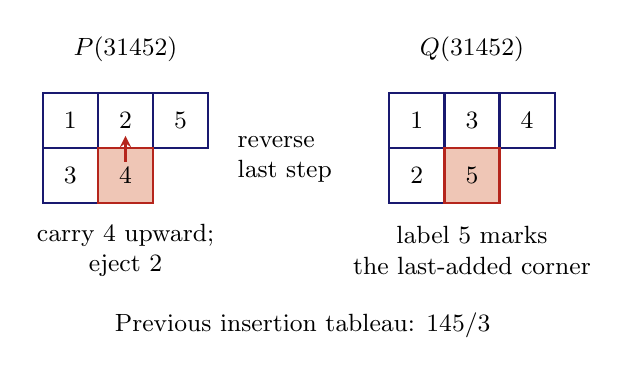
\begin{tikzpicture}[font=\small,>=stealth]
\foreach \x/\name in {0/P,4.4/Q}{
 \node at (\x+1.05,0.55) {$\name(31452)$};
 \foreach \j in {0,1,2}{\draw[MidnightBlue,thick] (\x+0.7*\j,0) rectangle (\x+0.7*\j+0.7,-0.7);}
 \foreach \j in {0,1}{\draw[MidnightBlue,thick] (\x+0.7*\j,-0.7) rectangle (\x+0.7*\j+0.7,-1.4);}
 \fill[BrickRed!20] (\x+0.7,-0.7) rectangle (\x+1.4,-1.4);
 \draw[BrickRed,thick] (\x+0.7,-0.7) rectangle (\x+1.4,-1.4);
}
\foreach \j/\v in {0/1,1/2,2/5}{\node at (0.7*\j+0.35,-0.35) {$\v$};}
\foreach \j/\v in {0/3,1/4}{\node at (0.7*\j+0.35,-1.05) {$\v$};}
\foreach \j/\v in {0/1,1/3,2/4}{\node at (4.4+0.7*\j+0.35,-0.35) {$\v$};}
\foreach \j/\v in {0/2,1/5}{\node at (4.4+0.7*\j+0.35,-1.05) {$\v$};}
\draw[->,BrickRed,thick] (1.05,-0.88) -- (1.05,-0.55);
\node[anchor=west,align=left] at (2.35,-0.85) {reverse\\last step};
\node[align=center] at (1.05,-2.0) {carry $4$ upward;\\eject $2$};
\node[align=center] at (5.45,-2.0) {label $5$ marks\\the last-added corner};
\node at (3.3,-2.95) {Previous insertion tableau: $145/3$};
\end{tikzpicture}
